

\section{Technologie wykorzystane w aplikacji}
\subsection{Klika słów wstępu.}
Jak wszyscy wiemy jedną z pierwszych dezycji projektanta jest wybór technologii, 
wykorzystywanych w tworzonej przez niego aplikacji. Dezycja ta znacząco wpływa na kształt naszego dzieła,
może też sprawić, że aplikacja będzie wyglądała bardzo nowocześnie i działała sprawnie. Ale z drugiej strony 
konsekwencje niewłaściwego wyboru też mogą być znaczące. Użytkownik chce aby jego polecenia były wykonywane
sprawnie a obsługa nie stwarzała problemów.

Współczene aplikacje internetowe są coraz bardziej rozbudowane i swym wyglądem oraz użytecznością nie ustępują
miejsca klasycznym aplikacjom. Nie dziwi więc niekogo fakt że taka aplikacja to złożony twór który łączy ze 
sobą wiele technologii. Niemal w każdej aplikacji tego tymu możemy natrafić na bazę danych, kontener servletów
czy też model. W najbliższych rozdziałach postaram się przybliżyć klika technologii obecnie stowsowanych do 
towrzenia aplikacji internetowych. Zaczniemy od najniższego poziomu czyli od bazy danych i stopniowo 
przejdziemy do ostatecznego widoku aplikacji, czyli tego z czego korzysta użytkownik. Zanim jednak zaczniemy 
opisywać technologie należy wspomniech o architekturze tego typu aplikacji.

\subsection{Architektura trójwarstwowa}
Jest arcitekturą typu klient serwer. Aplikacja podzielona jest na warstwy co umożliwia łatwiejsze
zarządzanie i modyfikacje programu. Dzięki temu możemy wprowadzać zmiany w jednenej z warstw bez konieczności
modyfikacji w innych warstwach. Schemat tej architekrury został przedstawiony na rysunku \ref{architekturaTrojwarstwowaRysunek}.
\begin{figure}[h]\centering

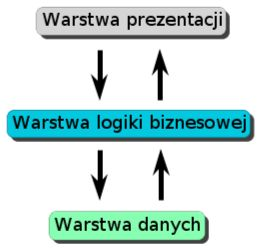
\includegraphics[scale=0.5]{architekturaTrojwarstwowa.jpg}
\caption{Schemat architektury trójwarstwowej}
\label{architekturaTrojwarstwowaRysunek}
\end{figure}
\subsubsection{Warstwa danych}
Służy do przechowywania, tworzenia zapytań i zarządzania danymi w aplikacji. Składa się z bazy danych oraz 
modułów, bibliotek zapewniających programiście wygodne API. Spośród wielu rozwiązań dostępnych na rynku 
ciekawym wydaje się open source'owy projekt jakim jest PostgreSQL. Natomiast aby możliwa była wygodna, szybka
i bezpieczna współpraca z bazą danych należy się zastanowić nad narzędziem zapewniającym translację między 
relacyjnym światem bazy danych a światem obiektowym. Przykładem takiego narzedzia może być framework Hibernate.
\subsubsection{Warstwa logiki biznesowej}
Warstwa odpowiedzialna za komunikację pomiędzy poszczególnymi warstwami ale również wykonuje obliczenia
i przygotowuje odpowiedzi do warstwy prezentacji. Powinna również realizować całą logikie biznesową aplikacji.
Warstwę tą można zrealizować przy pomocy szkieletu aplikacyjnego jakim jest ObjectLedge. Warstwa da zwraca
również odpowiedzi do warstwy prezentacji. Jak wiadomo niemożliwe jest w takim przypadku
stworzenie statycznej strony i jej wyświetlanie, ponieważ w aplikacji ciągle zachodzą pewne zmiany, które
muszą mieć odzwiercedlenie w warstwie prezentacji. Należy zatem generować strony dynamicznie. 
 Istnieje wiele
narzędzi do generowania dynamicznych stron HTML. Jednym z takich narzedzi jest projekt open source o nazwie
Velocity.

\subsubsection{Warstwa prezentacji}

Jedyna widoczna dla użytkownika warstwa. Daje mu możliwość dokonywania zmian w aplikacji oraz wyświetla
informacje o aktualnym stanie w jakim aplikacja się znajduje. Powinna być prosta, przejrzysta a także 
logiczna w obsłudze. W przypadku aplikacji internetowych zazwyczaj jest napisana z wykorzystaniem
technik takich jak HTML, JavaScript oraz  w celu ułatwienie stosowane są różne biblioteki napisane 
w JavaScripcie takie jak: Dojo czy JQuery.

\subsection{PostgreSQL}
Jak wszyscy wiemy w niemal każdej aplikacji mamy kontakt z danymi. Dane te są w różny sposób przetwarzane i 
katalogowane. W przypadku małej ilości możemy zapisać ja np. w pliku na dysku ale co zrobić gdy danych jest 
więcej i zapanowanie nad ich przechowywaniem i przetwarzaniem staje się uciążliwe. W takich przypadkach
z pomocą przychodzą sysatemy zarządzania bazami danych. Obecnie na rynku jest ich wiele i niemal każdy z liczących
się producentów oprogramowania posiada i promuje swój produkt. Projektant aplikacji staje przed bardzo trudnym 
zadaniem wyboru odpowiedniego systemu zarządzania bazą danych. Od jego wyboru zależy to ile czasu będzie musiał
poświęcić na uruchomienie i przyswojenie metod pracy z bazą danych. Jednym z takich systemów do zarządania bazą
danych jest PostgreSQL.

PostgreSQL początkowo nazwany Postgres powstał w 1986 i wywodzi się z wcześniejszego projektu o nazwie Ingres.
Twórcą tego systemu jest Michael Stonebraker. Jest to jeden z najpopularniejszych systemów do zarządania 
bazą danych, do jego popularności z pewnością przyczynił się fakt że jest on udostępniany na licencji BSD.
Licencja BSD (Berkeley Software Distribution License) umożliwia twórcom oprogramowania nie tylko użytkowanie 
tego systemu bez wnoszenia opłat ale również pozwala na tworzenie własnych modyfikacji w kodzie systemu 
PostgreSQL i rozprowadzanie bez konieczności załączania kodu źródłowego. Dodatkowym atutem tego systemu jest
fakt że możemy używać go na niemal każdym współczesnym systemie operacyjnym. 

System ten jest zgodny ze standardem SQL92, a obecnie implementuje większość ze standardu SQL:2008.
W systemie tym mamay możliwość używania wszyskich typów znajdujących się z standardzie SQL a także 
całe mnóstwo nowych typów specyficznych dla PostgreSQL. Na szczególną uwagę zasługują takie typy jak point, line 
czy box. Typy te mogą być w przydatne w przypadku wszelkiego rodzaju obliczeń geometryczno-karotgrafcznych,
co może zaciekawić wielu osoby pracujące na tego typu danych. Z kolei dla administratrów sieci PostgreSQL
również przygotował specjalne typy danych do których należą cidr czy inet. Jakby tego było mało PosgreSQL
pozwala na zdenifniowanie przez użytkownika własnego typu, który będzie przez niego używany.

Oprócz typów danych w bazie danych ważne jest co można z tymi danymi zrobić i tu też PostgreSQL pokazuję
że w tej kwestji może wiele począwszy od operwtorów, gdzie oprócz standarodwych posiada także takie jakich 
nie znajdziemy w żadnej innym systemie bazodanowym. Wśród niecodziennych operatorów możemy znaleźć
operatory służące do liczenia pola figury czy też uzyskiwania danych z adresów internetowych. Oczywiście tak
jak w przypadku typów danych PostgreSQL daje nam również możliwość towrzenia własnych operatorów. 
Do pracy z danymi wykorzystywane są również różnego rodzaju procedury wbudowane oraz funkcje, których w 
PostgreSQL-ie też jest mnóstwo. 

PostgreSQL ma również swoje ograniczenia, które w przypadku większości aplikacji (nawet tych dużych)
nie stanowią problemów. Podstawowe ogrniczenia bazy danych to:
\begin{table}[h]\centering
\caption{Ograniczenia PostgreSQL}
\label{postgresOrganiczeniaTable}
\begin{tabular}{|c||c|}
 \hline \textbf{Ograniczenie} & \textbf{Wartość} \\
 
 \hline
 \hline Maksymalny rozmiar bazy danych & nieograniczony \\
 \hline Maksymalny rozmiar tabeli & 32TB\\
 \hline Maksymalny rozmiar wiersza & 1.6TB\\
 \hline Maksymalny rozmiar pola & 1GB\\
 \hline Maksylalna liczba wierszy tabeli & nieograniczona\\
 \hline Maksylalna liczba kolumn w tabeli & 250 - 1600 w zależności od typów kolumn\\
 \hline Maksymalna liczba indeksów tabeli & nieograniczona\\ 
 \hline
\end{tabular}
\end{table}

\subsection{Objectledge}
Szkielet aplikacyjny umożliwiający tworzenie internetwych aplikacji w języku Java. Jest to projekt 
oparty na technologii PicoContainera i wykorzystujący wstrzykiwanie zalażności. Składa się z kilku 
modułów, które pozwalają na stworzenie pełnoprawnej aplikacji. ObjectLedge jest posiada licencję 
typu open source dzięki czemu możemy wykorzystywać go do tworzenia własnego oprogramowania, z 
zastrzeżeniem konieczności dołączenia informacji o prawach autorskich.
\subsubsection{MVC}
ObjectLedge wykorzystuje wzorzec projektowy MVC (Model Widok Kontroler). Moduł ten umożliwia oddzielenie 
warstwy widoku od warstwy dostępu do danych i działania na nich. Model w ObjectLedge jest częścią 
niewidoczną dla użytkownika, dostęp do niej ma jednynie programista tworzący aplikację. W większości 
przypadków w tej części aplikacji dostaję się do bazy danych i dokonuje modyfikacji. Kolejną warstwą 
jest Kontroler, jest on odpowiedzialny za przygotowywanie widoków oraz wykonywanie akcji zleconych 
przez użytkownika. Implementacja tej części znajduję się w klasach ActionExecutorValve oraz 
BuilderExecutorValve. Widok odpowiada za część aplikacji widoczną dla użytkownika. W ObjectLedge
jest on tworzony przy pomocy klas dziedziczących po klasie Bulider oraz wykorzystując mechanizm szablonów
taki jak np. Velocity.
\subsubsection{Security}
Moduł pozwalający na stworzenie zabazpieczeń w aplikacji. Zapewnia mechanizm autoryzacji oraz umożliwia 
wprowadzenia podziału na różne grupy użytkowników aplikacji. Moduł ten operra się o zdefiniowanie potencjalnych
użytkonikow aplikacji oraz ról jakie mogą posiadać. W zależności od zdefiniowanych w bazie danych ograniczeń
przypisanych do konkretnego użytkownika ObjectLedge zezwala lub nie na wykonanie danej operacji.
\subsubsection{Intake}
Moduł ten pozwala na połączenie formularzy w widoku z klasami znajdującymi się w modelu. Dzięki temu
możemy również sprawdzać czy dane wprowadzone przez użytkownika są poprawne. Sprawdzenie może odbyć się
poprzez zdefiniowanie pewnych cech jakie powinny posiadać wprowadzone dane ale również możemy zdenifiować
wyrażenia regularne jakie muszą spelniać dane zapisane przez użytkownika.
\subsection{Hibernate}
Hibernate jest narzędziem, które znacząco ułatwia pracę programiście pracującym z bazą danych, poprzez 
umożliwienie mu mapowania obeitowo-relacyjnego. 
Dzięki Hibernate możemy w łatwy sposób zmapować istniejący w bazie danych relacyjny model na model obiektowy
z ktorego programista korzysta w swojej aplikacji. Jedną z zalet tego frameworka jest to że współpracuje 
z większością baz danych obecnych na rynku i ma bardzo rozbudowane API, które pozwala użytkownikowi na wiele.
Za wykorzystniem tego frameworka w aplikacjach przemiawia również fakt że jest to projekt open sourcowy dzięki
czemu możemy z niego korzstać nie odpłatnie.

Hibernate to właściwie zbiór projektów służących do pracy z bazami danych, Hibernate składa się z następujących 
podprojektów:
\begin{description}
  \item[Hibernate Shards] Ułatwia pracę z wieloma bazami danych i daje możliwość pracy z wieloma bazami danych
  poprzez standardowe API.
  \item[Hibernate Search] Umożliwia pełnotekstowe wyszukiwanie.
  \item[Hibernate Tools] Zestaw narzędzi umożliwiających integrację ze środowiskiem Eclipse. Najważniejszą 
  i najbardziej przydatną funkcją jest możliwość generowania bazy danych na podstawie obiektów napisanych w
  języku java.
  \item[Hibernate Validator] Daje większe możliwości używania adnotacji w projekcie.
  \item[Hibernate Metamodel Generator] 
  \item[Hibernate OGM ]
\end{description}

Mapowanie obiektów odbywa się z wykorzystaniem 
odpowiednich plików xml w których definiujemy na jakie tabele w bazie danych mapujemy nasze obiekty w
aplikacji. Definiowane są w nim również powiązania między tabelami w bazie danych jak i również 
powiązania w modelu znajdującym się w aplikacji.
 Hibernate nie tylko pozwala nam w łatwy i przyjemny sposób zarządzać danymi w bazie danych ale również
przyspiesza odwołania do bazy danych poprzez buforowanie.

Hibernate umożliwia torzenie zapytań na trzy różne sposoby. Pierwszym z nich jest używanie wbudowanego
w Hibernate języka HQL, który składniowo jest podobny do standardowego SQL-a. Kolejnym sposobem wykonywania
zapytań jest użyawnie do tego celu SQL-a, zaś ostatni ze sposobow dostępu do bazy danych to używanie 
kryteriów.

W Hibernate istnieją dwa sposoby łączenia bazy danych z modelem w języku java. Pierwszy ze sposobów to
stworzenie na początku bazy danych a nastpnie na jej podstawie stowrzenie modelu w javie. Druga metoda jest 
odwrotna czyli na początku tworzymy model w naszej aplikacji a następnie Hibernate generuje schemat
bazy danych.
\subsection{Ajax}
Ajax jest to zbiór technik umożliwiających towrzenie stron, które swoim działaniem przypominają bardziej 
aplikacje uruchamiane bezpośrednio na komputezrze użytkownika niż aplikacje internetowe. Po raz pierwszy
technologia ta została wykorzystana w roku 2005 i wywołała spore zamieszanie na rynku. 
 Główną zaletą jest 
możliwość wprowadzania zmian w wyświetlanej stronie bez konieczności przeładowywania całego dokumentu. Nazwa
Ajax to skrót od Asynchronous JavaScript and XML, sugeruje to że wymiana danych pomiędzy przeglądarką a 
serwerem ma charakter asynchroniczny. Takie rozwiązanie powoduje że użytkownik nie musi czekać na odpowiedź
z serwera po wykonaniu jakiejś, natomiast może sobie spokojnie dalej używać aplikacji.

Ajax to właściwie zbiór już istniejących techlologii WWW, takich jak: HTML, CSS, XML, JavaScript. Połączenie
tych dało nowe możliwości dla twórców stron WWW.
 Ajax do komunikacji z serwerem używa obiektów XMLHttpRequest.

\subsection{Velocity}
Jest to procesor szblonów umożliwiający tworzenie dynamicznych stron WWW. Projekt ten jest typu open source
dzięki czemu możemy go używać w aplikacjach bez konieczności uiszczania opłat. Velocity wykorzystuje wzorzec
MVC dzieki czemu mamy lepiej podzieloną aplikacje. 
\subsection{JQuery}

\subsection{Dojo}
\newpage
\begin{thebibliography}{szerokosc}
\bibitem{postgreSQLDybikowski}Dybikowski Z.: PostgreSQL, Helion, Gliwice, 2001
\bibitem{postgresStronaDomowa}http://www.postgresql.org/about/
\bibitem{hibernateWAkcji}Bauer C. King G.: Hibernate w akcji, Helion, Gliwice, 2007
\bibitem{RozporzadzenieFaktury}Rozporządzenie Ministra Finansów z dnia 28 marca
2011 r.
w sprawie zwrotu podatku niektórym podatnikom, wystawiania faktur, sposobu ich
przechowywania oraz listy towarów i usług, do których nie mają zastosowania
zwolnienia od podatku od towarów i usług. (Dz.U. 2011 nr 68 poz. 360)
\end{thebibliography}